%\documentclass[twocolumn, trackchanges]{aastex6}
\documentclass[twocolumn]{aastex6}


\bibliographystyle{aasjournal}
\usepackage{graphicx}
\usepackage[suffix=]{epstopdf}
\usepackage{natbib}
\usepackage{amsmath}
\usepackage{url}
\usepackage{xspace}



%    Make Scientific Notation
\providecommand{\e}[1]{\ensuremath{\times 10^{#1}}}

% make the word Kepler italicized, deal w/ floating space afterwards
\newcommand{\Kepler}{\textsl{Kepler}\xspace}

\begin{document}

%%%%%%%%%%%%%%%%%%%%%%
\title{The GALEX View of ``Boyajian's Star''}

\shorttitle{GALEX View of ``Boyajian's Star''}
\shortauthors{Davenport et al.}

\author{
	James R. A. Davenport\altaffilmark{1,2},
	Kevin R. Covey\altaffilmark{1},
	Riley W. Clarke\altaffilmark{1}, \\
	Zachery Laycock\altaffilmark{1},
	Scott W. Fleming\altaffilmark{3},
	Tabetha S. Boyajian\altaffilmark{4},
	Benjamin T. Montet\altaffilmark{5,6},\\
	Bernie Shiao\altaffilmark{3},
	Chase C. Million\altaffilmark{7},
	David J. Wilson\altaffilmark{8},
	Manuel Olmedo\altaffilmark{9},
	Eric E. Mamajek\altaffilmark{10,11}
	}

\altaffiltext{1}{Department of Physics \& Astronomy, Western Washington University, 516 High St., Bellingham, WA 98225, USA}
\altaffiltext{2}{NSF Astronomy and Astrophysics Postdoctoral Fellow}
\altaffiltext{3}{STScI, 3700 San Martin Dr., Baltimore, MD 21218}
\altaffiltext{4}{Department of Physics and Astronomy, Louisiana State University, 261-A Nicholson Hall, Tower Dr, Baton Rouge, LA 70803}
\altaffiltext{5}{Department of Astronomy and Astrophysics, University of Chicago, 5640 S. Ellis Ave, Chicago, IL 60637, USA}
\altaffiltext{6}{NASA Sagan Fellow}
\altaffiltext{7}{Million Concepts LLC, PO Box 119, 141 Mary St, Lemont, PA 16851, USA}
\altaffiltext{8}{Department of Physics, University of Warwick, Coventry CV4 7AL, UK}
\altaffiltext{9}{Instituto Nacional de Astrof\'{i}sica Optica y Electr\'{o}nica, Tonantzintla, Puebla, M\'{e}xico}
\altaffiltext{10}{Jet Propulsion Laboratory, California Institute of Technology, 4800 Oak Grove Drive, Pasadena, CA 91109, USA}
\altaffiltext{11}{Department of Physics \& Astronomy, University of Rochester, Rochester, NY 14627, USA}



%%%%%%%%%%%%%%%%%%%%%%%%%%%%%%
\begin{abstract}
{\bf rewrite!}
The enigmatic star KIC 8462852, also known as ``Boyajian's Star'',  has puzzled for both its short (days) length dimming events, and a years-long secular dimming observed by the \Kepler mission.
GALEX provides both short timescale sampling from the photon-counting data, and longer baseline data from multiple campaigns that imaged this field/ also providing a wide wavelength baseline to compare with the optical \Kepler data, and provide important constraint for models of this system.
here we investigate both the short and long timescale data. from 4 GALEX visits totaling 1600 seconds of exposure time in 2011, spread over 70 days, we find no coherent NUV variability in the system on 10--100 sec timescales during these time windows. Comparing the integrated flux from these 2011 visits to the 2012 NUV flux published in the GALEX-CAUSE Kepler survey, we find a 3\% decrease in brightness of KIC 8462852. This decrease is the first  validation of the secular fading reported by \citet{montet2016} not in optical wavelengths. The similar amplitudes between the NUV and optical data rule out typical interstellar dust as the cause of this fading.
\end{abstract}



%%%%%%%%%%%%%%%%%%%%%%%%%%%%%%
\section{Introduction}
KIC 8462852, also known as ``Boyajian's Star'', is an unusual F3 dwarf in the \Kepler field that has exhibited unexplained optical variability on a variety of timescales. The initial discovery was of several dramatic, short timescale (days) dimming events with amplitudes up to 20\% in the \Kepler 30-min cadence data \citep{boyajian2015}. Though the \Kepler mission \citep{borucki2010} obtained data at a 30-min cadence for $\sim$4 years on this star, no definitive pattern or cycle was found, nor has any single explanation for this variability been accepted by the community \citep{wright2016b}.

Analysis of archival optical photographic plates has found that KIC 8462852 may have additionally faded nearly 16\% over the past century \citep{schaefer2016}. Such a precise measurement for a single star is difficult, and the result has been debated \citep{hippke2016}. However, using the 53 ``Full Frame Images'' (FFIs) spread over the 4-year \Kepler mission, \citet{montet2016} were able to trace the brightness of KIC 8462852 using an independent flux calibration. The resulting flux-calibrated FFI light curve showed definitively that KIC 8462852 faded by more than 3\% over 4 years. A years-long timescale variability, with possible periodicity, has recently been confirmed with an analysis of archival ground-based optical photometry \citep{simon2017}.

The short (days) and long (years) timescale variability discovered for KIC 8462852 has presented a unique set of observational constraints on any single model used to describe the system. For example, if variable dust extinction is responsible for both temporal features, then it must have a wildly variable density distribution on small spatial scales, and a small density gradient over large spatial scales. Searches for an infrared flux excess consistent with a foreground or circumstellar dust shell have to date found no strong detection \citep{marengo2015}.


Since optical variability alone has not produced a single explanation for KIC 8462852, multi-wavelength studies are needed to constrain nature of the long timescale fading and short timescale dimming. Follow-up multi-band photometric and spectroscopic campaigns are underway\footnote{\url{http://www.wherestheflux.com}}, which will provide an improved understanding of any future ``dips''. However, to date no contemporaneous, multi-wavelength  measurement of the mysterious variability for KIC 8462852 has been available.


Archival photometry at ultraviolet wavelengths from the GALEX mission \citep{galex} is now available, and provides an important new dataset for understanding KIC 8462852. This data includes NUV monitoring over a range of time baselines, from seconds to more than a year. Time-tagged photon data has recently been made available for GALEX \citep{million2016}, including a Python toolkit to search for and interact with this high cadence data product called {\tt gPhoton} \citep{gphoton}. This allows us to resample all available GALEX survey data into any desired cadence. In the case of KIC 8462852, GALEX had $\sim$1600 seconds of data available from four separate visits spread across a $\sim$70 day baseline in 2011. In \S\ref{sec:short} we analyze this NUV data with {\tt gPhoton} sampled at a 10 second cadence, and over the whole 70 day period.




The \Kepler field was revisited by GALEX during a special campaign, dubbed the GALEX-CAUSE Kepler (hereafter GCK) survey. This survey occurred in 2012, and overlapped a portion of the Quarter 14 operations of the original \Kepler mission. Using a ``scan'' observing mode that differed from the standard GALEX survey, the GCK catalog had 1413.8 seconds of data available for KIC 8462852, which was combined into a single stacked exposure of this region \citep{olmedo2015}. Unfortunately, since the observing mode differed from the standard GALEX survey, this GCK data is not available for analysis with {\tt gPhoton} presently. In \S\ref{sec:long} we explore the long timescale evolution of KIC 8462852 between the 2011 and 2012 visits, and compare directly to the observed fading by \citet{montet2016}.

In \S\ref{sec:dust} we discuss possible interpretations for the nature of KIC 8462852 that the combined \Kepler and GALEX observations provide, including an estimate of the dust extinction properties necessary to reproduce the long timescale NUV observations. Finally in \S\ref{sec:summary} we summarize this work, and discuss the potential utility of GALEX in the study of other rare and unusual variable \Kepler objects.


%%%%%
\begin{figure}[!t]
\centering
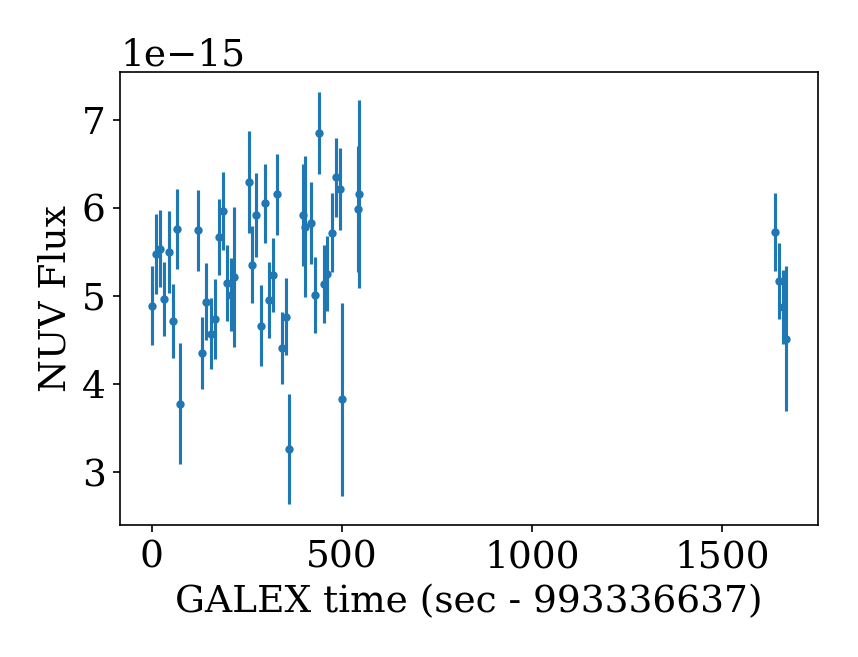
\includegraphics[width=2.7in]{KIC8462852_0_lc}
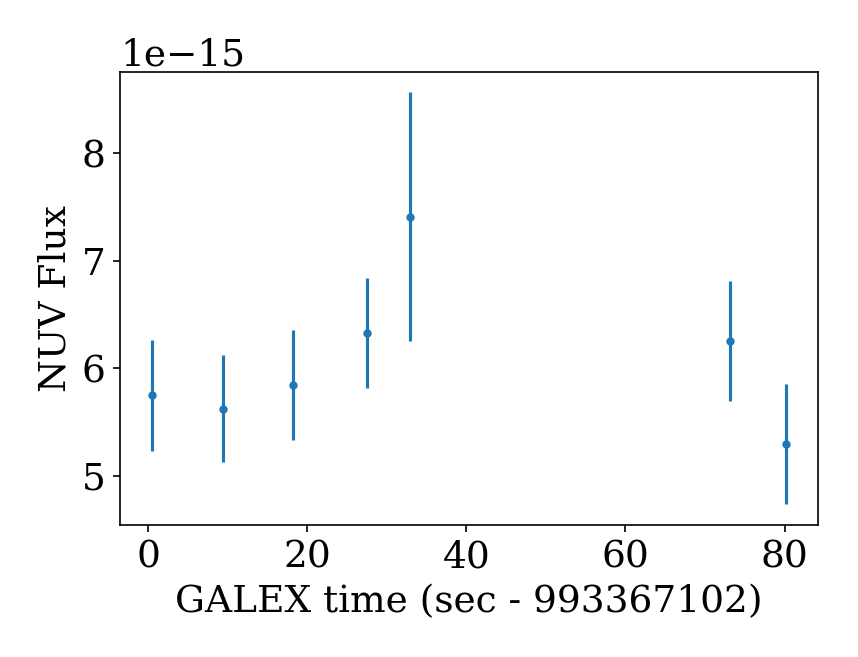
\includegraphics[width=2.7in]{KIC8462852_1_lc}
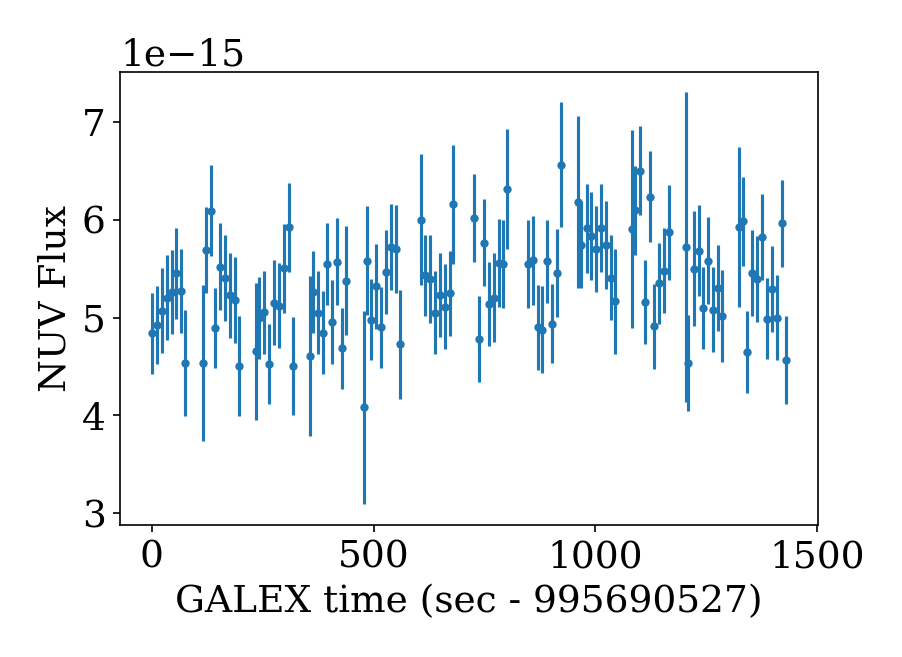
\includegraphics[width=2.7in]{KIC8462852_2_lc}
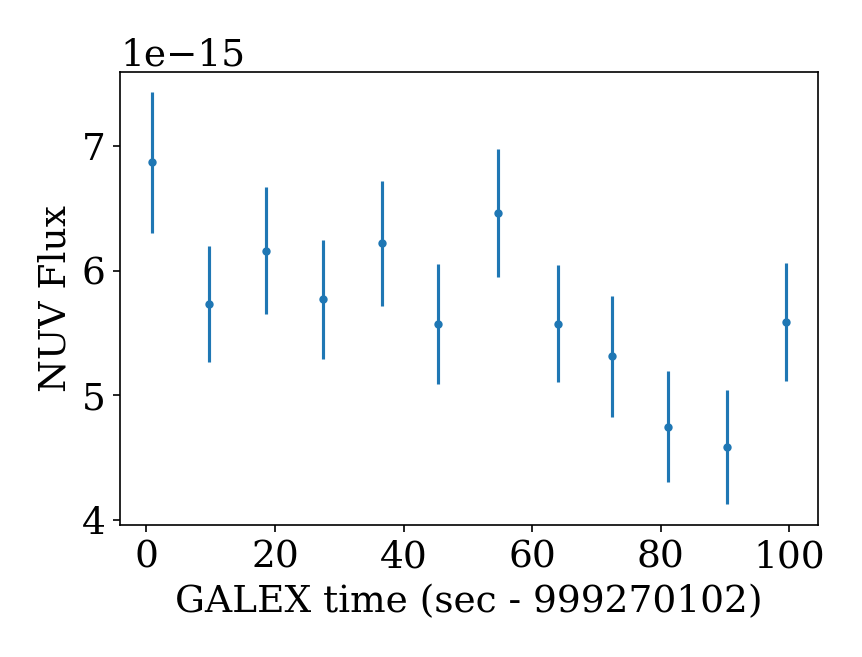
\includegraphics[width=2.7in]{KIC8462852_3_lc}
\caption{
Light curves from {\tt gPhoton} sampled at a 10-second cadence for the 4 visits in 2012. All epochs are shown (grey), while those having no photometric warning flags set are highlight (blue). Error bars shown are the photometric errors for each point computed by {\tt gPhoton}.}
\label{fig:shorttime}
\end{figure}



%%%%%%%%%%%%%%%%%%%%%%
\section{Short Timescale Variability}
\label{sec:short}

Within each of the four GALEX visits available for KIC 8462852, we searched for short timescale variability using {\tt gPhoton}. While nano-second optical variability has been investigated for this target \citep{abeysekara2016}, few other studies have looked at variability on timescales shorter than the 30-minute cadence available with \Kepler.
The four GALEX visits in 2011 ranged from $\sim$70 to $\sim$1400 seconds in duration. Data for each visit was sampled at a 10-second cadence, as shown in Figure \ref{fig:shorttime}. Small amplitude variability is apparent in several of the visits, with coherent structure over durations of approximately 60-100 seconds. Computing a Lomb-Scargle periodogram using {\tt gatspy} \citep{gatspy}, we find moderate power with a broad peak at around 80-seconds. This appears to be due to the $\sim$120 second observing cycle of the GALEX instrument in the standard ``Petal Pattern'' observing mode, and we believe is not astrophysically significant.
A periodic signal of 0.88 days was found in \Kepler, which was presumed by \citet{boyajian2015} to be due to the rotation of starspots in- and out-of view on the surface of KIC 8462852. However, the four GALEX visits shown in Figure \ref{fig:shorttime} are too short to capture this rotation signature, and thus our GALEX data are not able to explore variability at this timescale.




Since the standard GALEX data for this target was spread over four separate visits, we also examined the medium-timescale variability over $\sim$70 days. In Figure \ref{fig:medtime} we show the median flux from within each of the {\tt gPhoton}-processed visits. The uncertainties shown in Figure \ref{fig:medtime} are computed as the standard deviation in the 10-sec sampled data within each visit, and are $\sim$10x larger than the statistical error on each visit's median flux. Unfortunately this 70-day time window did not correspond to any of the previously identified dimming events from \citet{boyajian2015}. Though there is scatter between these four visits in Figure \ref{fig:medtime}, no significant coherent variability is seen on this intermediate timescale with GALEX.


%%%%%
\begin{figure}[!t]
\centering
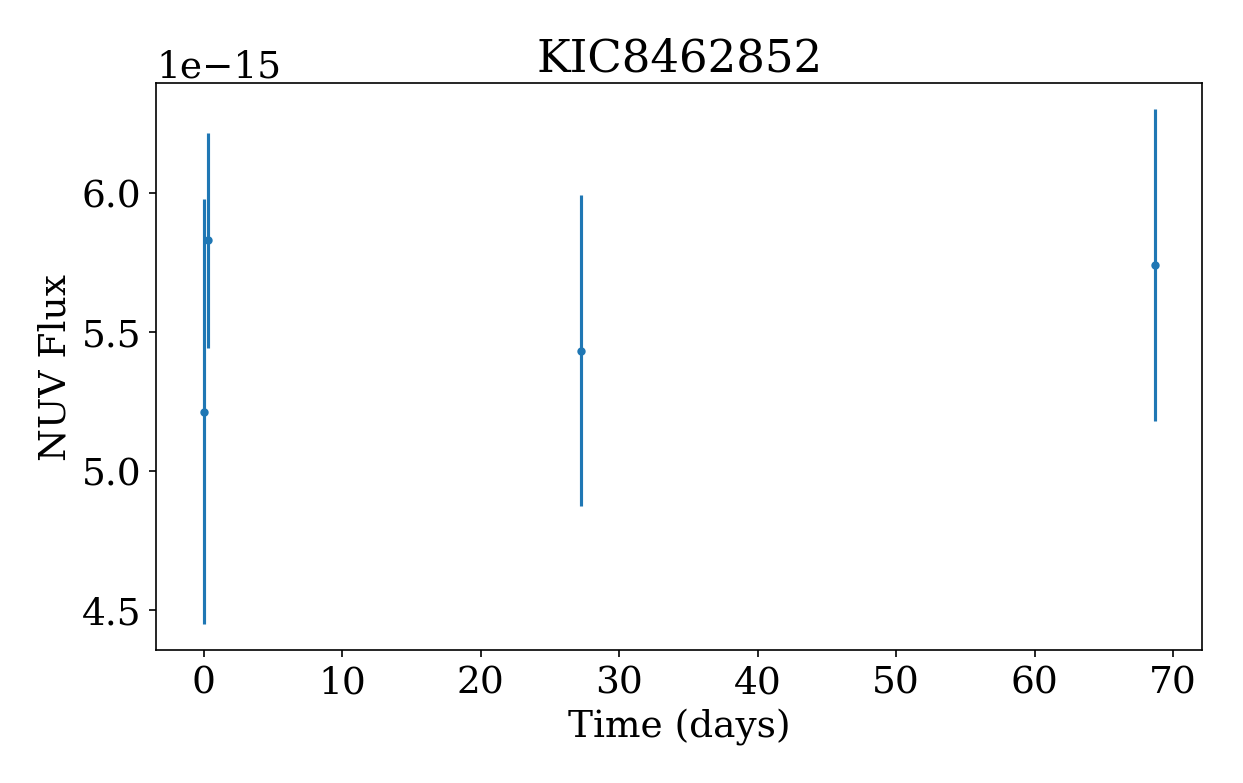
\includegraphics[width=3.5in]{KIC8462852}
\caption{Median flux within each of the four visits spaced over $\sim$70 days in 2011 by GALEX. Uncertainties shown are the standard deviation in flux within each 10-sec sampled {\tt gPhoton} light curves from Figure \ref{fig:shorttime}. No significant change in flux is seen over this 70 day window.
}
\label{fig:medtime}
\end{figure}





%%%%%%%%%%%%%%%%%%%%%%
\section{Long Timescale Variability}
\label{sec:long}


While the standard GALEX survey data available within {\tt gPhoton} only sampled $\sim$70 days within 2011, the \Kepler field was fortunately re-observed with GALEX in 2012. As part of the GALEX Complete All-Sky UV Survey Extension (CAUSE) program, 104 square degrees within the \Kepler field were re-observed in the NUV, creating the GALEX-CAUSE Kepler survey (GCK). This GCK data was obtained using a drift-scan mode, which was processed using a custom pipeline, and is therefore not available for photon-counting analysis with the {\tt gPhoton} toolkit at this time. A catalog of the integrated fluxes and uncertainties for 475,164 \Kepler targets observed in GCK, including for KIC 8462852, was made available by \citet{olmedo2015}.


In Figure \ref{fig:longtime} we present the GALEX data for this target as observed in 2011 and 2012. The 2011 data represents the final GALEX GR6 catalog flux value for KIC 8462852 of $16.46 \pm 0.01$ mag from \citet{bianchi2014}, while the 2012 data is from the GCK data of $16.499\pm0.006$ mag from \citet{olmedo2015}. Both data were converted to fluxes, and then were normalized to the flux of the 2011 visit. For comparison we also show the slow fading discovered in the \Kepler FFI's by \citet{montet2016}. Note: the fact that the GALEX and \Kepler FFI data are normalized to a relative flux of 1 around 2011 (MJD$\sim$55700) is a coincidence. However, the fact that the GALEX flux decays coherently with the \Kepler FFI flux over this time baseline is significant. Importantly, this is the first multi-wavelength confirmation of the slow fading reported by \citet{montet2016} for KIC 8462852.



%%%%%
\begin{figure}[!t]
\centering
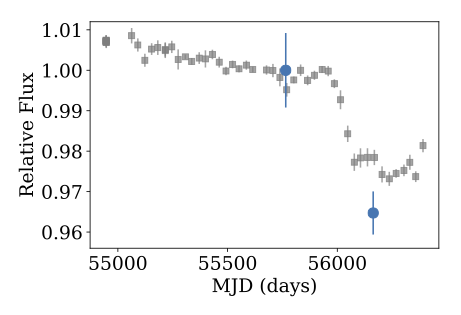
\includegraphics[width=3.5in]{KIC8462852_compare}
\caption{
Comparison of the 2011 and 2012 fluxes for KIC 8462852 as measured by GALEX (blue circles), with the \Kepler FFI data shown in \citet{montet2016} as reduced with the new ``f3'' package from \citet{montet2017} for comparison (grey squares). The amplitude of variability over this time window is nearly identical between the two surveys.
}
\label{fig:longtime}
\end{figure}






%%%%%%%%%%%%%%%%%%%%%%
\section{Implications for the Nature of KIC 8462852}
\label{sec:dust}

While many explanations for the nature of KIC 8462852 have been proposed, there is effectively no consensus on the nature of the years-long timescale fading (or variability) observed by \citet{montet2016} and confirmed here. Critically, with only a single wavelength band available from \Kepler, and no apparent characteristic timescale for this variation with the 4-year observing window, little can be constrained from the \Kepler data alone. \citet{metzger2017} have argued the long-timescale fading could be due to stellar atmosphere recovery after a planetary in-spiral, and possibly the short-timescale dips are due to remaining debris. \citet{montet2016} note the fading in the \Kepler FFI's may be due to the transit of a dust cloud. However none of these models definitively explain the long-timescale variability observed in \citet{montet2016}.  


By combining the optical \Kepler FFI light curve with the long-timescale GALEX NUV data presented here, we can place the first multi-wavelength constraints on KIC 8462852. A natural model to compare the simultaneous variability in the NUV and optical is that of a dust cloud. Extinction by dust in the interstellar medium is well studied, and several models with varying dust compositions are available at these wavelengths. Regardless of {\it where} the dust originates (i.e. circumstellar versus interstellar), such extinction models are a useful path forward in exploring the fading of KIC 8462852.

To demonstrate the impact dust would have in these two bands, we computed the extinction in the GALEX NUV band that would be predicted given the fading observed by \citet{montet2016} within the 2011 and 2012 time windows observed by GALEX. We used a standard \citet{cardelli1989} dust model with $R_V=3.1$, computed using the Python code from \citet{barbary2016}. The comparison of this prediction with the flux decrease observed by GALEX is shown in Figure \ref{fig:dust}. The \citet{cardelli1989} model over-predicts the fading found in the NUV, indicating the fading is more gray (less wavelength dependent) that a standard $R_V=3.1$ dust model. This rules out ``normal'' interstellar dust as the culprit of the fading observed by \citet{montet2016}.


%%%%%
\begin{figure}[!t]
\centering
\includegraphics[width=3.5in]{KIC8462852_extinction_model_1}
\caption{Comparison between the flux decrease observed at the effective wavelengths of the GALEX NUV and \Kepler bands (blue solid line) and a corresponding $R_V=3.1$ dust model from \citet{cardelli1989} tuned to pass through the \Kepler data (orange dashed line). The standard dust model over-predicts the NUV flux decrease given the observed \Kepler fading.}
\label{fig:dust}
\end{figure}


However, the NUV response of dust models is highly dependent on grain composition. This can be explored in standard dust models by modifying the $R_V$ parameter. We then tuned a dust model to match both the observed \Kepler optical and GALEX NUV dimming by varying the $R_V$ and specific extinction ($A_V$) parameters. To fit the fading in both wavelengths simultaneously requires a dust model with  $R_V=5.0\pm0.9$. This is not typical for interstellar extinction material, such a high $R_V$ has been reported for example around young protostars \citep[e.g.][]{hecht1982}. Note also that competing dust models can produce significantly different NUV extinctions. For example, by modeling the \Kepler and GALEX fading for KIC 8462852 shown in Figure \ref{fig:longtime} with a \citet{fitzpatrick2009} dust model, we find a best-fit parameter of $R_V=5.8\pm1.6$.


If the slow fading is indeed due to the transit of a dust cloud, we can further put a constraint on how much dust should be present. Based on relations from \citep{guver2009}, we find that an extinction of $A_V = 0.026$ mag  needed to fit the fading with the \citet{cardelli1989} dust model  corresponds to a column density of $N_H\sim5\e{19}$ cm$^{-2}$ . Similarly, using the relations from \citet{rachford2002} that have some dependence on dust composition ($R_V$), we find an estimated column density $N_H\sim4.0\e{19}$ cm$^{-2}$  given $A_V = 0.026$ and $R_V=5.08$. However, this high of a column density poses an intriguing challenge given the lack of warm circumstellar dust detection by \citet{thompson2016}.



%%%%%%%%%%%%%%%%%%%%%%
\section{Summary}
\label{sec:summary}

explored short timescale variability with {\tt gPhoton} on seconds timescales, and on 70 day window. nothing significant at NUV wavelengths.

using 2011 and 2012 detections with GALEX we have provided the first independent verification of slow fading of this target

though the long timescale light curve is very sparsely sampled, the combination of NUV and optical wavelengths provides a powerful constrain on the nature of this slow dimming. 

In the hunt for other objects of this class, we are able to expand our search criteria beyond the dramatic short timescale events and slow dimming observed with \Kepler, to now include slow variability in the NUV. 

new papers: \citep{meng2017} (new extinction, confirms our Rv), simon2017 (no long-term effect, but confirms slow fading over this timescale), %rappaport2017 (exocomets may explain short timescale dips)

%%%%%%%%%%%%%%%%%
\acknowledgments
JRAD is supported by an NSF Astronomy and Astrophysics Postdoctoral Fellowship under award AST-1501418. 

Work by B.T.M. was performed under contract with the Jet Propulsion Laboratory (JPL) funded by NASA through the Sagan Fellowship Program executed by the NASA Exoplanet Science Institute.

DJW has received funding from the European Research Council under the European Union�s Seventh Framework Programme (FP/2007-2013)/ERC Grant Agreement n. 320964 (WDTracer). 

Part of this research was carried out at the Jet Propulsion Laboratory, California Institute of Technology. under a contract with the National Aeronautics and Space Administration. This document does not contain export controlled information.


%%%%%%%%%%%%%%%%%
\bibliography{/Users/james/Dropbox/references.bib}

\end{document}
